% 学院全称及教师归属于 2026-09-09 对照学院官网；F-MAP-04 的公开名称位点已补齐。
% 来源：https://it.xju.edu.cn/xygk/xyjj.htm；https://it.xju.edu.cn/info/1144/3131.htm
\CasmTopic{1. 工作基础}{（与本课题相关的研究工作积累和已取得的研究工作成绩）}

% 内容来源：NSFC_2027_Mapping/extraTex/3.1.研究基础.tex
\subsection*{1.1\quad 与本项目相关的研究工作积累}

申请人长期从事多模态学习、跨模态检索与遥感视觉理解研究，已有工作在三个方面与本项目直接衔接。

\subsubsection*{1.1.1\quad 跨模态检索的表征与匹配}

申请人在跨模态检索方向的工作直接支撑本项目内容二。代表性成果为 Feature Fusion Mamba Hashing via Decoupling for Cross-Modal Retrieval（\textit{IEEE Signal Processing Letters}, 2026, 33: 609--613），申请人为通讯作者，负责研究构思、方法设计、实验指导、结果分析及论文撰写与修改。该工作围绕跨模态哈希检索中的特征融合与解耦展开，使申请人对图文双塔的表征学习、相似度构造、负样本组织与检索评测流程具备完整的实操经验。相关的跨模态检索工作还包括 Dual-Branch Feature-Fused and Multi-Semantic Aligned Hashing for Supervised Cross-Modal Retrieval（ICASSP 2026），申请人为通讯作者。

上述通用跨模态哈希检索工作为内容二的对齐或重排序实现提供经验；关系证据的状态判定仍需在本项目中验证。

\subsubsection*{1.1.2\quad 遥感图像语义与空间结构理解}

申请人在遥感视觉理解方向积累了对遥感影像语义、空间结构与多模态交互的处理经验。代表性成果包括 RSHR+: Progressive Question-Conditioned Visual Calibration and Structured State-Space Reasoning for Remote Sensing Visual Question Answering（\textit{Expert Systems with Applications}, 2026, 328: 132953，申请人为通讯作者，负责研究构思、方法设计、实验指导、结果分析及论文撰写与修改）与 RSSR: Efficient Knowledge Transfer and Deep Spatial Modeling for Remote Sensing Visual Question Answering（\textit{Computer Vision and Image Understanding}, 2026, 268: 104753，申请人为通讯作者）。两项工作分别涉及遥感影像的渐进式视觉校准、结构化状态空间推理与深度空间建模，使申请人熟悉遥感影像中地物尺度差异大、背景占比高、空间格局复杂等固有特点。

上述工作以视觉问答为任务载体，其语义与空间结构建模经验可用于本项目的遥感图文双向检索。

\subsubsection*{1.1.3\quad 多模态表征与知识引入}

申请人在多模态表征学习方面的工作包括 Knowledge-Aware Image Understanding with Multi-Level Visual Representation Enhancement for Visual Question Answering（\textit{Machine Learning}, 2024, 113(6): 3789--3805），申请人为第一作者兼通讯作者，负责研究构思、方法设计、实验指导、结果分析及论文撰写与修改；以及 SPCA-Net: A Spatial Position Relationship Co-Attention Network for Visual Question Answering（\textit{The Visual Computer}, 2022），申请人为第一作者。后者围绕空间位置关系的协同注意力建模展开，与本项目关注的空间关系主题在技术手段上有直接承接关系。


\subsection*{1.2\quad 可行性分析}

\subsubsection*{1.2.1\quad 两条积累恰好构成本项目所需的能力组合}

内容一的三态判定需要辨认遥感影像中的空间关系，并判断关系证据对图文匹配的作用。RSHR+ 与 RSSR 提供遥感影像空间结构与视觉校准经验，跨模态哈希检索工作提供表征学习、相似度构造与负样本组织经验，SPCA-Net 则提供空间关系进入多模态交互的实现经验。内容三所需的分层评测、等预算对照与消融设计，可沿用申请人在既有工作中形成的实验组织方法。

\subsubsection*{1.2.2\quad 关于前期基础的边界}

目前尚无可直接复用于本项目的专属数据、代码、模型配置、评价脚本或消融实验日志。公开数据集仅完成发布页面与获取入口核验，尚未下载，也未开展完整性检查与抽样审计。数据审计、关系词表、三态标注规范、关系挑战子集及基线复现均安排在执行期内建立。已发表成果支撑方法与工程能力，尚不构成本项目科学假说的实验证据；具体对应关系见图~\ref{fig:foundation-mapping}。

% F12: F12_积累与需求对位-v3.png
% 与后续正文合排，避免单独居中的插图页产生大面积留白。
\begin{figure}[!htb]
    \centering
    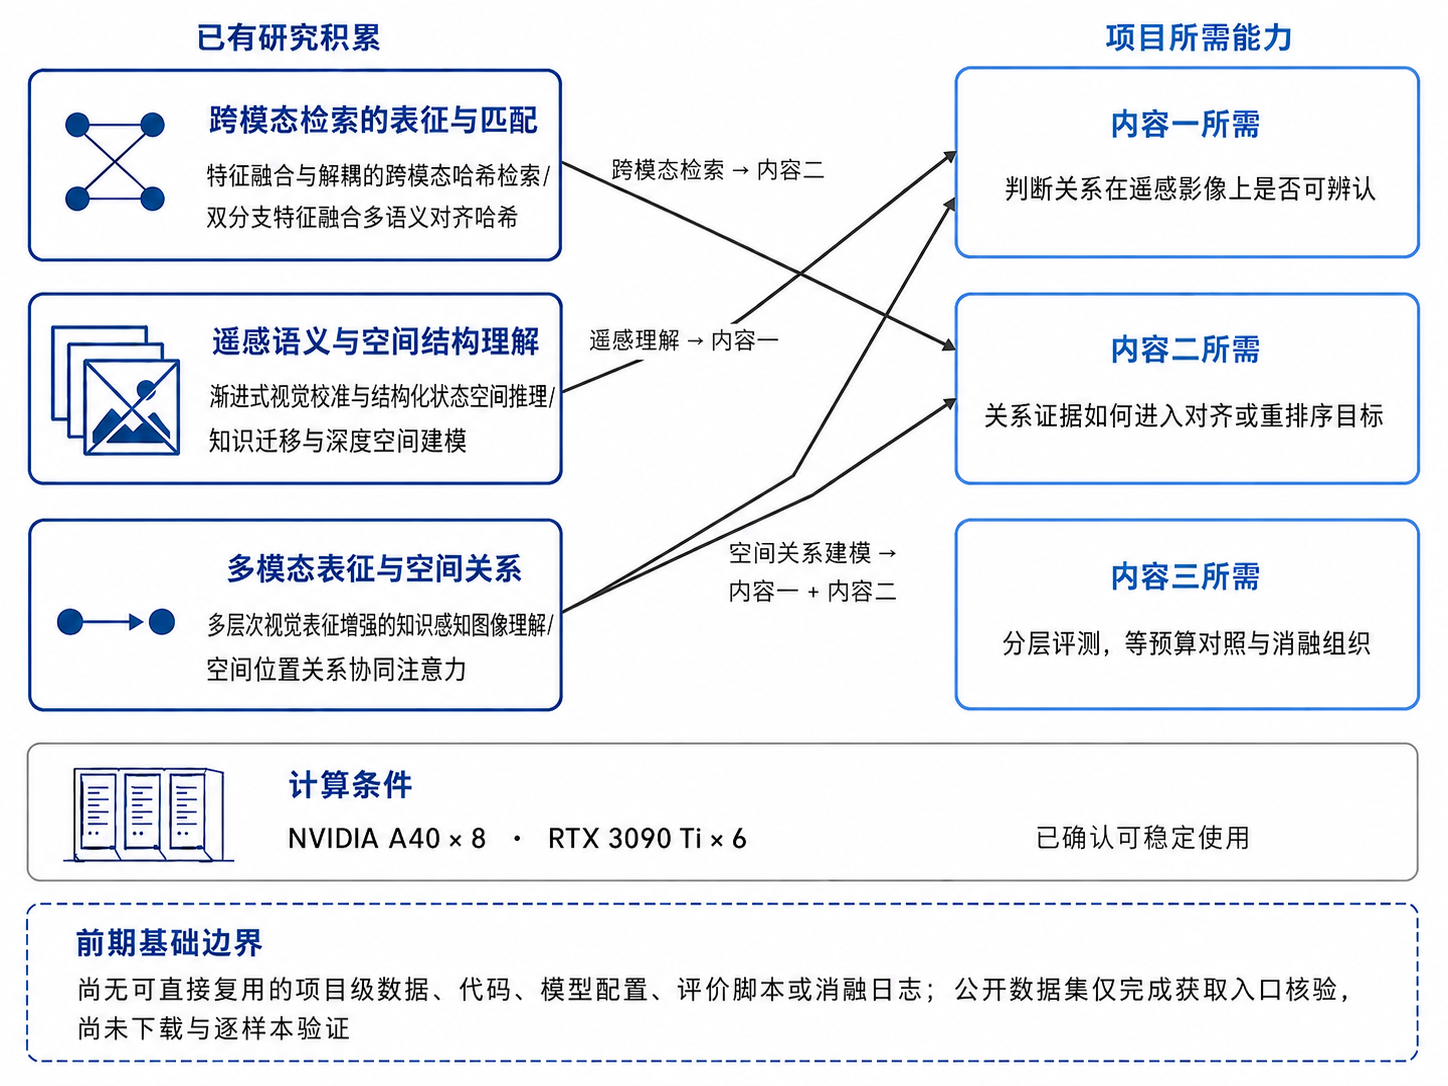
\includegraphics[width=\linewidth]{figures/F12_积累与需求对位-v3.png}
    \caption{申请人积累与项目需求对位。已有成果支撑方法与工程能力，项目专属数据、代码和验证材料仍需在执行期内建立。}
    \label{fig:foundation-mapping}
\end{figure}


\CasmTopic{2. 工作条件}{（包括已具备的实验条件）}

% 内容来源：NSFC_2027_Mapping/extraTex/3.2.工作条件.tex
\subsection*{2.1\quad 已具备的实验条件}

\subsubsection*{2.1.1\quad 计算条件}

申请人已确认可稳定使用的计算资源包括 NVIDIA A40 图形处理器 8 块与 NVIDIA GeForce RTX 3090 Ti 图形处理器 6 块。本项目采用参数高效适配策略控制可训练参数规模，不依赖超大规模集群；上述资源可支撑中等规模视觉语言模型的领域适配、三臂受控对照，以及每组实验不少于 3 个随机种子的重复运行与多组消融的排队执行。

\subsubsection*{2.1.2\quad 软件与工程条件}

申请人具备 Linux、Python、主流深度学习框架、Git 与 \LaTeX{} 工具链的完整使用经验；在软件系统研发、数据治理与科研工程化方面的积累，可直接用于本项目的数据审计流程、标注工具搭建、实验日志管理与轻量检索演示开发。

\subsubsection*{2.1.3\quad 数据条件}

本项目使用公开遥感图文数据。RSITMD\cite{yuan2022amfmn} 与 RSICD\cite{lu2018rsicd} 的作者仓库提供影像、标注文件与解析程序的获取入口，此前核验时入口有效；必要且许可条件满足时，可使用 SkyScript\cite{wang2024skyscript} 作小规模补充验证。项目按使用现有公开数据规划，不安排商业数据采购或大规模实地采集；实际获取、许可范围与关系覆盖程度的核验安排见第 2.2.1 节。

\subsubsection*{2.1.4\quad 团队与依托单位条件}

申请人为新疆大学副教授、硕士研究生导师，创建并负责 ALPHA Group 研究团队，具备指导研究生开展系统性研究的基础。依托单位新疆大学在计算机与人工智能方向具备相应的学科平台与研究生培养条件，申请人所在二级单位为计算机科学与技术学院（网络空间安全学院）。

\subsection*{2.2\quad 尚缺少的实验条件及拟解决的途径}

\subsubsection*{2.2.1\quad 数据许可条款与关系覆盖程度尚需落实}

此前已核验三个数据集的获取入口：RSITMD 的标注文件与解析脚本由作者仓库分发，影像另经网盘入口提供；RSICD 的标注文件托管于作者仓库，影像包经云盘入口获取；SkyScript 提供对象存储直链，核验时响应正常。完整下载、文件校验和使用权限仍需在启动阶段落实。

此前核验中，RSITMD 与 RSICD 的作者仓库未声明开源许可，只提出引用原始论文的要求；RSICD 的底图取自公开地图服务，可能附带第三方使用条款。SkyScript 仓库采用 MIT 许可，但影像和文本标签分别涉及 Google Earth Engine 与 OpenStreetMap 的来源条款。派生标注的公开再分发范围尚未确认，成果交付形式须据此确定。

目前尚无可判定空间关系占比及分层样本数量的实测结果。启动阶段由孔哲组织数据获取与完整性核对，桑乐整理去重后的描述，孔哲和张建宏完成 600 组审计及 100 条试标，申请人主持规范审定。审计须报告不同关系组的可判定比例、未知态原因、有效独立描述数量和试标一致性；重复描述只计一次证据，关系覆盖程度以实际审计结果为准。

\textbf{拟解决途径}：2027 年 1 月底前依据审计和试标形成可用关系类型、判定规范及抽样规则初版，4 月底前仅依据开发数据完成修订并冻结。若某类关系证据稀少或一致性不足，先在开发数据中复核规则并缩减关系范围，无法可靠判定的记录保留未知态；1800 条挑战记录为总体核验目标，分层覆盖与可检出的效应按实际样本报告。若审计仍不足以支撑三态机制检验，则转向关系冲突识别或覆盖度稳健性分析，交付审计、规范和对照结果。最终测试样本及其标签不随方法效果修改。许可不支持派生标注公开时，按获准范围交付索引、处理脚本与版本说明。

\subsubsection*{2.2.2\quad 关系证据的人工标注力量需要组织}

内容一按 1800 条挑战记录安排双人独立判定、一致性统计、争议仲裁和 10\% 随机抽查（达到目标规模时为 180 条）。由孔哲、张建宏承担两套独立标注，桑乐和于得武协助规范与工具，申请人主持仲裁并组织复核；正式标注前先完成 100 条试标培训。上述为执行期工作安排，目前尚未形成已完成的标注成果。

\textbf{拟解决途径}：依托 ALPHA Group 的 7 名参与研究生按既定分工推进，2026 年 11 月至 2027 年 1 月完成 600 组审计、100 条试标培训及首次开发回流；2--4 月结合开发数据继续试标，完成第二次规范修订并冻结；5--7 月完成 1800 条正式记录的双人核验、仲裁和 180 条抽查，封存标签，供 8--10 月一次性批量最终测试使用。工作量测算按每条每人约 10 分钟估算，正式独立判定约需 600 小时，另为审计、培训、仲裁、抽查和返修安排约 300 小时；该估算用于排期，不作为已发生工时。以现有 2 个集中助研岗位、各 6 个月的 1.20 万元劳务预算组织工作，投入月份按实际阶段任务安排，其他成员按职责提供工具和评测支持，不新增商业标注采购。

\subsubsection*{2.2.3\quad 补充算力的落实情况}

除申请人已确认可稳定使用的上述设备外，学院层面存在可申请的公共算力资源，但\textbf{固定账号、设备型号与使用额度尚未落实}，因此本申请仅将其作为补充条件列出，不作为稳定可用的实验条件计入。

\textbf{拟解决途径}：本项目的实验设计以已确认可用的设备为基准进行规划，不依赖补充算力即可完成既定研究任务；若后续获得学院公共算力的正式配额，将用于扩大消融实验的覆盖范围与随机种子数量，属于增量而非必要条件。

\subsection*{2.3\quad 利用研究基地的计划与落实情况}

本项目基于公开数据与申请人已确认可用的计算条件开展，暂无利用国家实验室、全国重点实验室或部门重点实验室的具体安排。后续如落实相关基地支持，可用于补充验证与学术交流。


\CasmTopic{3. 申请人及课题组主要成员简介}{（包括申请人和课题组主要成员的学历和研究工作简历，近期已发表与本课题有关的主要论著目录和获得学术奖励情况及在本课题中承担的任务）}

% 教育与工作经历依据共用申请人信息，并于 2026-09-07 对照个人主页；提交前本人终核。
\subsection*{3.1\quad 申请人基本情况与教育经历}

颜丰，男，1990 年 11 月出生，新疆大学副教授、硕士研究生导师，博士。2019 年 9 月至 2023 年 8 月在新疆大学计算机科学与技术专业攻读博士学位；2012 年 9 月至 2014 年 6 月在上海海事大学计算机技术专业攻读硕士学位；2008 年 9 月至 2012 年 6 月在海南热带海洋学院生态学专业完成本科学习并获得学士学位。

\subsection*{3.2\quad 研究工作简历}

2023 年 12 月起任新疆大学副教授，2023 年 10 月至 12 月在新疆大学从事教学与科研工作；2018 年 3 月至 2019 年 8 月在浙江大学山东工业技术研究院从事科研与技术工作；2016 年 10 月至 2017 年 12 月在上海中科软科技有限公司从事软件技术工作。上述经历形成了从软件系统研发、数据处理到多模态模型训练与实验评价的研究基础。

\subsection*{3.3\quad 在本课题中拟承担的任务}

申请人拟负责科学问题凝练与总体研究方案设计，组织地理实体关系词表与三态判定规范的制定，开展关系证据约束的匹配方法研究，负责对照实验与数据使用的质量控制，并组织论文撰写、成果整理及结题报告编制。每年工作时间为 7 个月，与申请信息表一致。

% 内容来源：NSFC_2027_Mapping/extraTex/3.1.研究基础.tex
\subsection*{3.4\quad 已取得的研究工作成绩}

申请人围绕多模态学习与遥感视觉理解形成了系列成果，包括发表于 \textit{Machine Learning}、\textit{Expert Systems with Applications}、\textit{Computer Vision and Image Understanding}、\textit{IEEE Signal Processing Letters}、\textit{Neural Networks}、\textit{The Visual Computer} 等期刊及 ICASSP 等会议的论文，相关代表作与本人贡献见本部分第 1.1 小节。申请人曾担任 \textit{Pattern Recognition}、\textit{Neural Networks}、\textit{Machine Learning} 等期刊审稿人。

申请人主持与参与了多项科研项目，其中与多模态方向相关的项目情况详见“研究基础与工作条件”第 4 小节。


\subsection*{3.5\quad 课题组主要成员与拟定分工}

% 身份依据：docs/applicants/00_参与者信息.md 及本项目 members.tex 的申请人确认记录。
% 未提供各人的教育起止年月、专业、既往研究经历及成果，不从学号或相邻项目分工推断。
本课题主要参与者为孔哲、张建宏、杨铄、孟星宇、桑乐、吕中原和于得武。7 人均为新疆大学在读硕士研究生，已获学士学位，无专业技术职称。各成员拟在申请人指导下承担下述任务。

孔哲：拟负责公开数据获取、许可与完整性核对、近重复去重及固定划分，并与张建宏独立完成关系样本核验。

张建宏：拟负责三态判定规范试标、关系挑战子集标注、一致性统计及争议样本整理，与孔哲交叉核验，由申请人主持争议仲裁。

杨铄：拟负责 CLIP、RemoteCLIP 基线复现和参数高效适配实验，维护一致的数据预处理、训练预算及运行配置。

孟星宇：拟负责关系约束匹配主线、三臂对照及等量随机屏蔽消融的实现，并整理训练稳定性分析结果。

桑乐：拟负责实体关系词表、描述覆盖分析和文本关系解析，维护影像坐标关系与数据增强标签同步规则。

吕中原：拟负责标准检索、关系挑战及覆盖度分档评测，实施等预算对照和去重后迁移测试，整理统计结果与错误归因。

于得武：拟负责代码整合、版本与实验日志管理、效率测试、复现材料和轻量检索演示，并协助成果归档。

申请人统筹研究问题、方法设计与质量核查，组织标注仲裁及结题成果审定。

\CasmTopic{4. 承担科研项目情况}{（申请人和课题组主要成员正在承担的科研项目情况，要注明项目的名称和编号、经费来源、起止年月、与本课题的关系及承担的具体工作内容等）}

% 内容来源：NSFC_2027_Mapping/extraTex/3.3.承担项目情况.tex
\subsection*{4.1\quad 申请人正在承担的与本项目相关的科研项目}

\subsubsection*{4.1.1\quad 多模态融合技术研究及其在新疆产业集群中的应用}

资助机构与项目类别：自治区天池英才引进计划（青年博士人才）。该项目无独立项目批准号，依据为项目任务书。获资助金额 50 万元，起止年月为 2025 年 2 月至 2028 年 2 月，申请人为主持人，负责总体研究方案、关键模型设计与成果组织。

与本项目的关系及负责内容：该项目面向多模态融合技术及其在区域产业中的应用，研究范围较宽；本申请聚焦于遥感图文检索这一具体任务中“描述不完备条件下地理实体关系证据的状态判定”这一科学问题，研究对象、拟解决的关键问题、使用数据与评测方式均与该项目不同，二者在经费与成果上分别独立核算，不存在重复申请或重复列支。

\subsubsection*{4.1.2\quad 数据驱动下基于互补型生成对抗网络与神经统计模型的公路沙害智能预警研究}

资助机构与项目类别：国家自然科学基金地区科学基金项目，批准号 62466056。项目获资助总额 32 万元，基金委系统登记单位为新疆大学，起止年月为 2025 年 1 月至 2028 年 12 月。申请人为参与者，负责数据的收集整理。

与本项目的关系及负责内容：该项目面向公路沙害智能预警，与本申请的遥感图文检索任务在科学问题与技术路线上均不相同；申请人在该项目中承担数据收集整理工作，与本申请的职责不重叠。

\subsubsection*{4.1.3\quad 可学习乘积量化与状态空间模型协同的长上下文高效注意力机制研究}

资助机构与项目类别：CAAI---蚂蚁科研基金，批准号 202604140006。项目获资助总额 15 万元，起止年月为 2026 年 2 月至 2027 年 2 月。申请人为参与者，负责高效注意力机制研究。

与本项目的关系及负责内容：该项目面向长上下文高效注意力机制，属模型效率方向的基础方法研究，不涉及遥感图文检索、地理实体关系建模与检索评测协议；其执行期在本申请执行期开始前后结束。

\subsection*{4.2\quad 主要参与者正在承担的与本项目相关的科研项目}

本项目 7 名研究生参与者的名单和本课题分工已列于前述成员简介及成员表，7 人均为在读硕士研究生，已获学位为学士，均无专业技术职称。拟参与的研究生均\textbf{无正在承担且与本申请相关的科研项目}。

\subsection*{4.3\quad 与本项目的区别与联系}

申请人正在承担的项目中，与本申请在技术领域上存在一定关联的是多模态融合方向的天池英才项目，其余项目在研究对象与科学问题上与本申请没有实质交叉。本申请与前者共享多模态表征学习这一技术基础，但研究对象从“区域产业应用中的多模态融合”收敛到“遥感图文检索中描述不完备条件下的关系证据状态判定”，科学问题、验证数据与成果形式均独立设置。

申请人承诺：不将立项前已形成的论文、模型或代码认定为本项目的阶段成果，不将同一成果重复列为多个项目的产出；成果归属边界以各项目任务书与成果标注为准。
